\documentclass[preview, beamer]{standalone}

\usepackage{tikz}
\usepackage{pgfplots}
\usepgfplotslibrary{fillbetween}

\usetikzlibrary{positioning, shadows, fit, arrows.meta, backgrounds, overlay-beamer-styles}


\begin{document}
\pgfplotsset{delpoint/.style={
			scatter,
			thick,
			mark=o,
			mark size=5pt,
			only marks,
			scatter,
		}}

% Define style for line plots
\pgfplotsset{delline/.style={
			mesh,
			thick,
			samples=50
		}}

\newcommand{\funcDel}[1]{100 * exp(-3 * #1 / 100)}
\def\tikzshadowopacityregister{1}
\resizebox{\textwidth}{!}{
	\begin{tikzpicture}[
			% genius way to fix shadows for invisble objectsa - credits to Symbol 1
			% https://tex.stackexchange.com/questions/357364/how-can-i-make-drop-shadows-appear-with-their-nodes-in-a-forest-tree-in-beamer
			invisible/.append code={\def\tikzshadowopacityregister{0}},
			every shadow/.style={opacity=\tikzshadowopacityregister},
			node distance=0.5cm,
			modelanchor/.style={minimum width=1cm, minimum height=1.5cm, inner sep=0},
			modelbox/.style={draw, rectangle, minimum width=1cm, inner sep=0, label={[rotate=90]center:model}, fill=white, drop shadow},
			imslice/.style={minimum height=1.5cm, inner sep=0, draw, rectangle, drop shadow},
			every arrow/.append style={ultra thick},
			>=Stealth
		]
		\pgfmathsetmacro{\pointAx}{0}
		\pgfmathsetmacro{\pointBx}{23}
		\pgfmathsetmacro{\pointCx}{100}

		\pgfmathsetmacro{\pointAy}{\funcDel{\pointAx}}
		\pgfmathsetmacro{\pointBy}{\funcDel{\pointBx}}
		\pgfmathsetmacro{\pointCy}{\funcDel{\pointCx}}
		\begin{axis}[
				%title={Deletion},
				xlabel={Perturbation Amount},
				ylabel={Predicted Class Probability},
				axis lines=left,
				xmin=-10, xmax=110,
				ymin=-10, ymax=110,
				xtick={0,100},
				ytick={0,100},
				legend pos=north west,
				%ymajorgrids=true,
				%grid style=dashed,
				%yticklabel style={rotate=90}, % Rotate y-axis labels by 45 degrees
				xticklabel=\pgfmathprintnumber{\tick}\%, % Add % sign to x-axis labels
				yticklabel=\pgfmathprintnumber{\tick}\%, % Add % sign to y-axis labels
				colormap={coolwarm}{
						rgb(0cm)=(0,0,1);
						rgb(1cm)=(1,0,0);
					},
				scatter src=y,
			]

			% Define a variable
			%\pgfmathsetmacro{\phi}{3}

			% Define a function
			%\pgfmathsetmacro{\f}{100 * exp(-\phi * x)}

			\only<3-6>{
				\addplot[delpoint]
				coordinates {
						(\pointAx, \pointAy)
					};
			}
			\only<7-9>{
				\addplot[delpoint]
				coordinates {
						(\pointAx, \pointAy)
						(\pointBx, \pointBy)
					};
				\addplot[delline, domain=0:23] {\funcDel{x}};
			}
			\only<10->{
				\addplot[delpoint]
				coordinates {
						(\pointAx, \pointAy)
						(\pointBx, \pointBy)
						(\pointCx, \pointCy)
					};
				\addplot[delline, domain=0:100] {\funcDel{x}};
			}
			\only<11>{
				\path[name path=axis] (axis cs:0,0) -- (axis cs:100,0);
				\addplot[name path=f, domain=0:100] {\funcDel{x}};
				\addplot [
					thick,
					color=blue,
					fill=blue,
					fill opacity=0.05,
					draw
				]
				fill between[
						of=f and axis,
						soft clip={domain=0:100},
					];
			}


			\node[inner sep=5pt] at (axis cs: \pointAx,\pointAy) (pointA) {};
			\node[inner sep=5pt] at (axis cs: \pointBx,\pointBy) (pointB) {};
			\node[inner sep=5pt] at (axis cs: \pointCx,\pointCy) (pointC) {};

		\end{axis}

		% MODEL ANCHORS
		\node[minimum width=1cm, minimum height=1.5cm] at (pointA -| 8, 0) (modelA) {};
		\node[minimum width=1cm] at (pointB -| 8, 0) (modelB) {};
		\node[minimum width=1cm, minimum height=1.5cm] at (pointC -| 8, 0) (modelC) {};

		% MODEL BOX
		\node[fit=(modelA)(modelB)(modelC), modelbox] (model) {};


		% INPUT A
		\node[right=of modelA, imslice, label=above:{AD Sample}] (inputA) {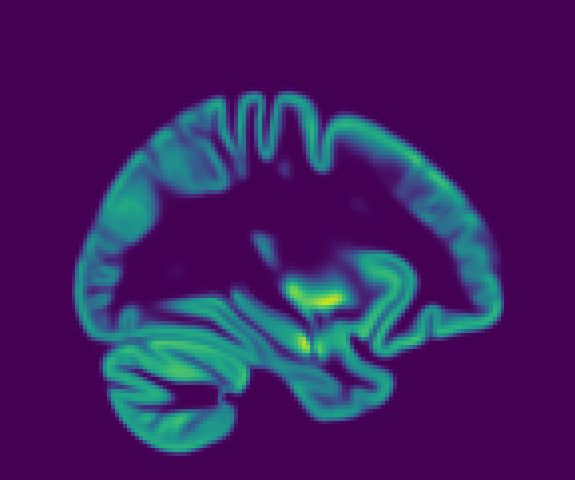
\includegraphics[height=1.5cm]{figures/ad_slice.png}};

		\draw[->, visible on=<2-4>] (inputA) -- (modelA);
		\draw[->, visible on=<3-4>] (modelA) -- node[pos=0.2] (router) {} (pointA);

		\node[draw, circle, fill, inner sep=1pt, visible on=<4>] at (router) {};

		\node[right=of inputA, imslice, label={[rotate=90, anchor=north, visible on=<4->]right:Attribution}, visible on=<4->] (map) {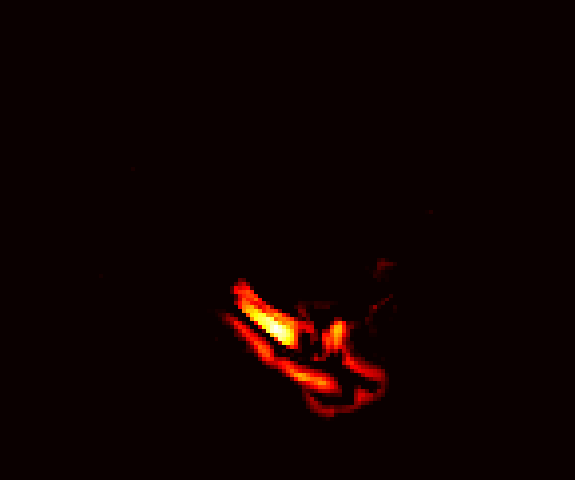
\includegraphics[height=1.5cm]{figures/ttest_slice.png}};
		\draw[->, visible on=<4>] (router.center) -- ++ (0,1.5cm) -| (map);

		% INPUT B
		\node[right=of modelB, imslice, visible on=<5->] (inputB) {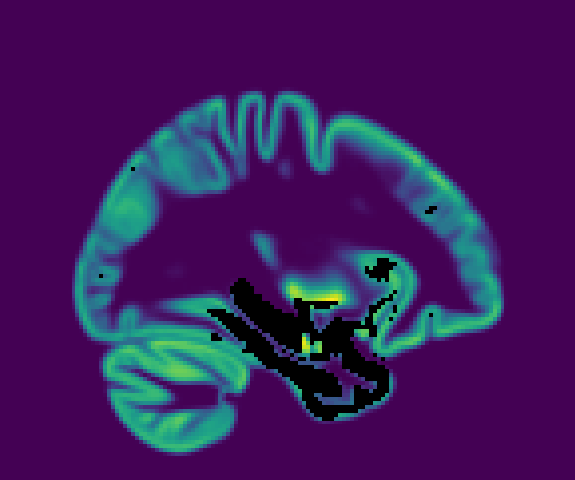
\includegraphics[height=1.5cm]{figures/ad23_slice.png}};
		\draw[->, visible on=<5->] (map) |- node[midway] (router2) {} (inputB);
		\node[visible on=<5->, label={[rotate=90, align=center, anchor=north, visible on=<5->]right:{perturbation}}] at (router2) {};
		\draw[->, visible on=<5->] (inputA) -- (inputB);

		\draw[->, visible on=<6-7>] (inputB) -- (modelB);
		\draw[->, visible on=<7>] (modelB) -- (pointB);


		% INPUT C
		\node[right=of modelC, imslice, visible on=<8->] (inputC) {
\includegraphics[height=1.5cm]{figures/ad100_slice.png}};

		\draw[->, visible on=<8->] (map) |- (inputC);
		\draw[->, visible on=<8->] (inputB) -- (inputC);
		\draw[->, visible on=<9-10>] (inputC) -- (modelC);
		\draw[->, visible on=<10>] (modelC) -- (pointC);

		% background layer does not work for some reason
		\begin{scope}
			\node[fit=(inputB)(inputC), draw, rectangle, dashed, visible on=<5->] {};
		\end{scope}
	\end{tikzpicture}
}
\end{document}